% Chapter3.tex
\chapter{WebDoc - Web Application Documentor}\label{ch:CP}

\begin{figure}[h]
    \centering
    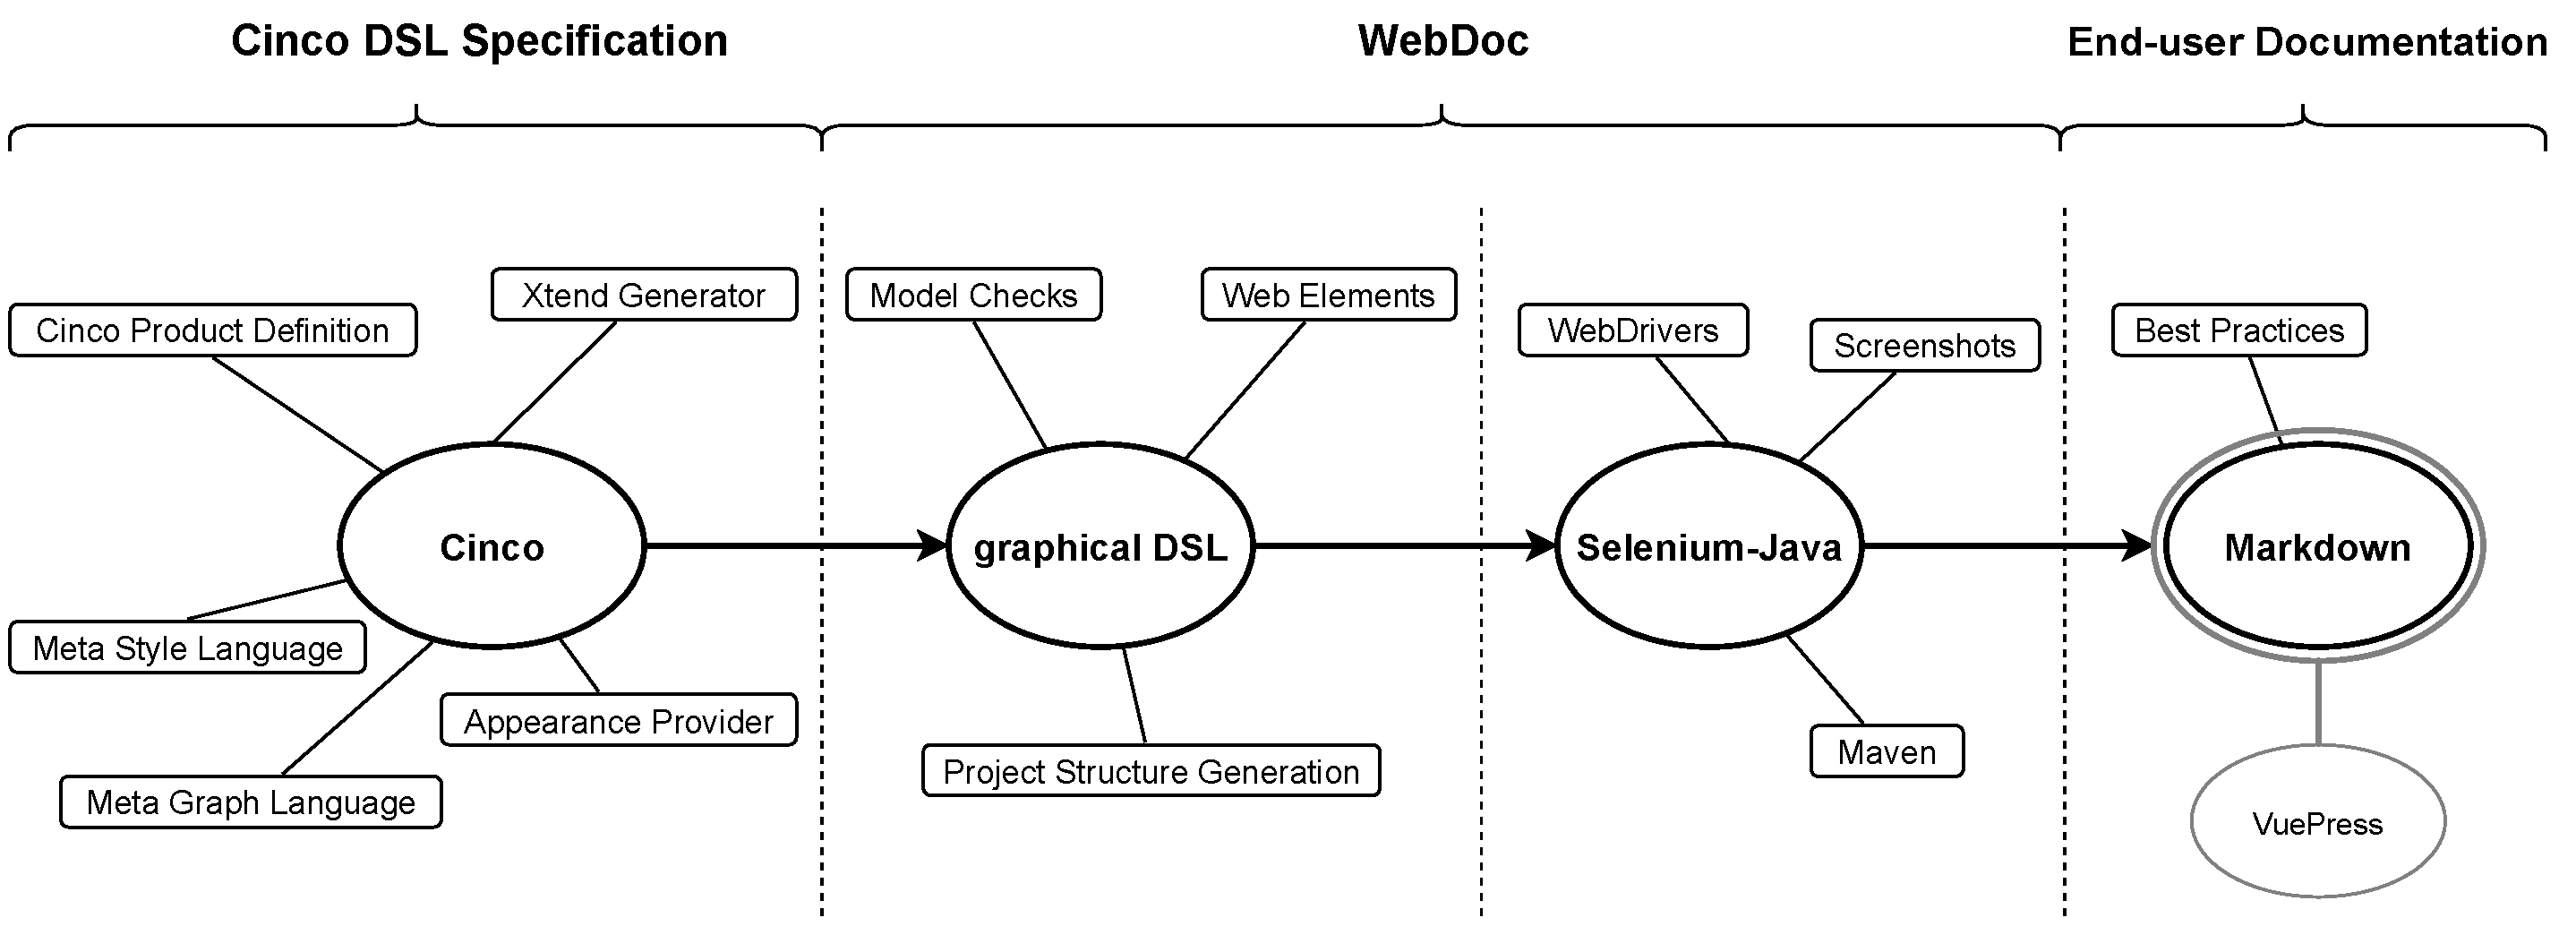
\includegraphics[width=\textwidth]{WebDocDevelopment-all.pdf}
    \caption{End user Documentation creation process workflow}
    \label{fig:procWorkflow}
\end{figure}

Having described the metalevel of the graphical modeling tool, we come now to the description of the model editor instantiated from it. The goal of this chapter is to explain the the appearance and behavior of the various model elements. First, we give a succinct definition of a graphical DSL, then illustrate the fundamental building blocks of our documentation model and by presenting at the same time the \textsc{Cinco} product application. Later on, we demonstrate the use of these graphical elements to specify the important configuration of the website we want to document. At the end, we show how using the editor built-in generator, a project structure, that constitute the target application, is generated.

\section{Graphical DSL}\label{sec:gDSL}

Our graphical DSL mainly comprises node elements, which have been applied different appearances to, in order to resemble to some extent the corresponding web elements they represent, as well as connector elements to connect the nodes to sequence graphs. The purpose behind this approximated replication is not to recreate all possible web elements, but to give the developer a sense of control over the interactable UI elements. With those elements at hand, the designer can simply model a user action by arranging node elements following the navigation path of the web application. This graphical language is in such way domain specific, that it is tailored for modeling web applications inside a web browser; modeling a documentation for a desktop application for example would not be possible.

\section{Graph Editor}\label{sec:graphEditor}

The editor is mainly composed of the canvas in the middle of the working environment (1), where the developer can drag and drop model elements from the palette located on the right-hand side (2). Herein, elements are grouped in a single category; this is achieved using the \lstinline[language=MGL]{@palette("category name")} annotation in the~.mgl meta-specification. On the left-hand side we have the project explorer showing the current project structure (3). The main model files have the extensions .doc and .feat, where the latter is the entry point of the documentation application. By hovering over a model element, an arrow symbol appears, allowing the developer to similarly drag and drop connecting edges from the source to the target element.

\begin{figure}[h]
    \centering
    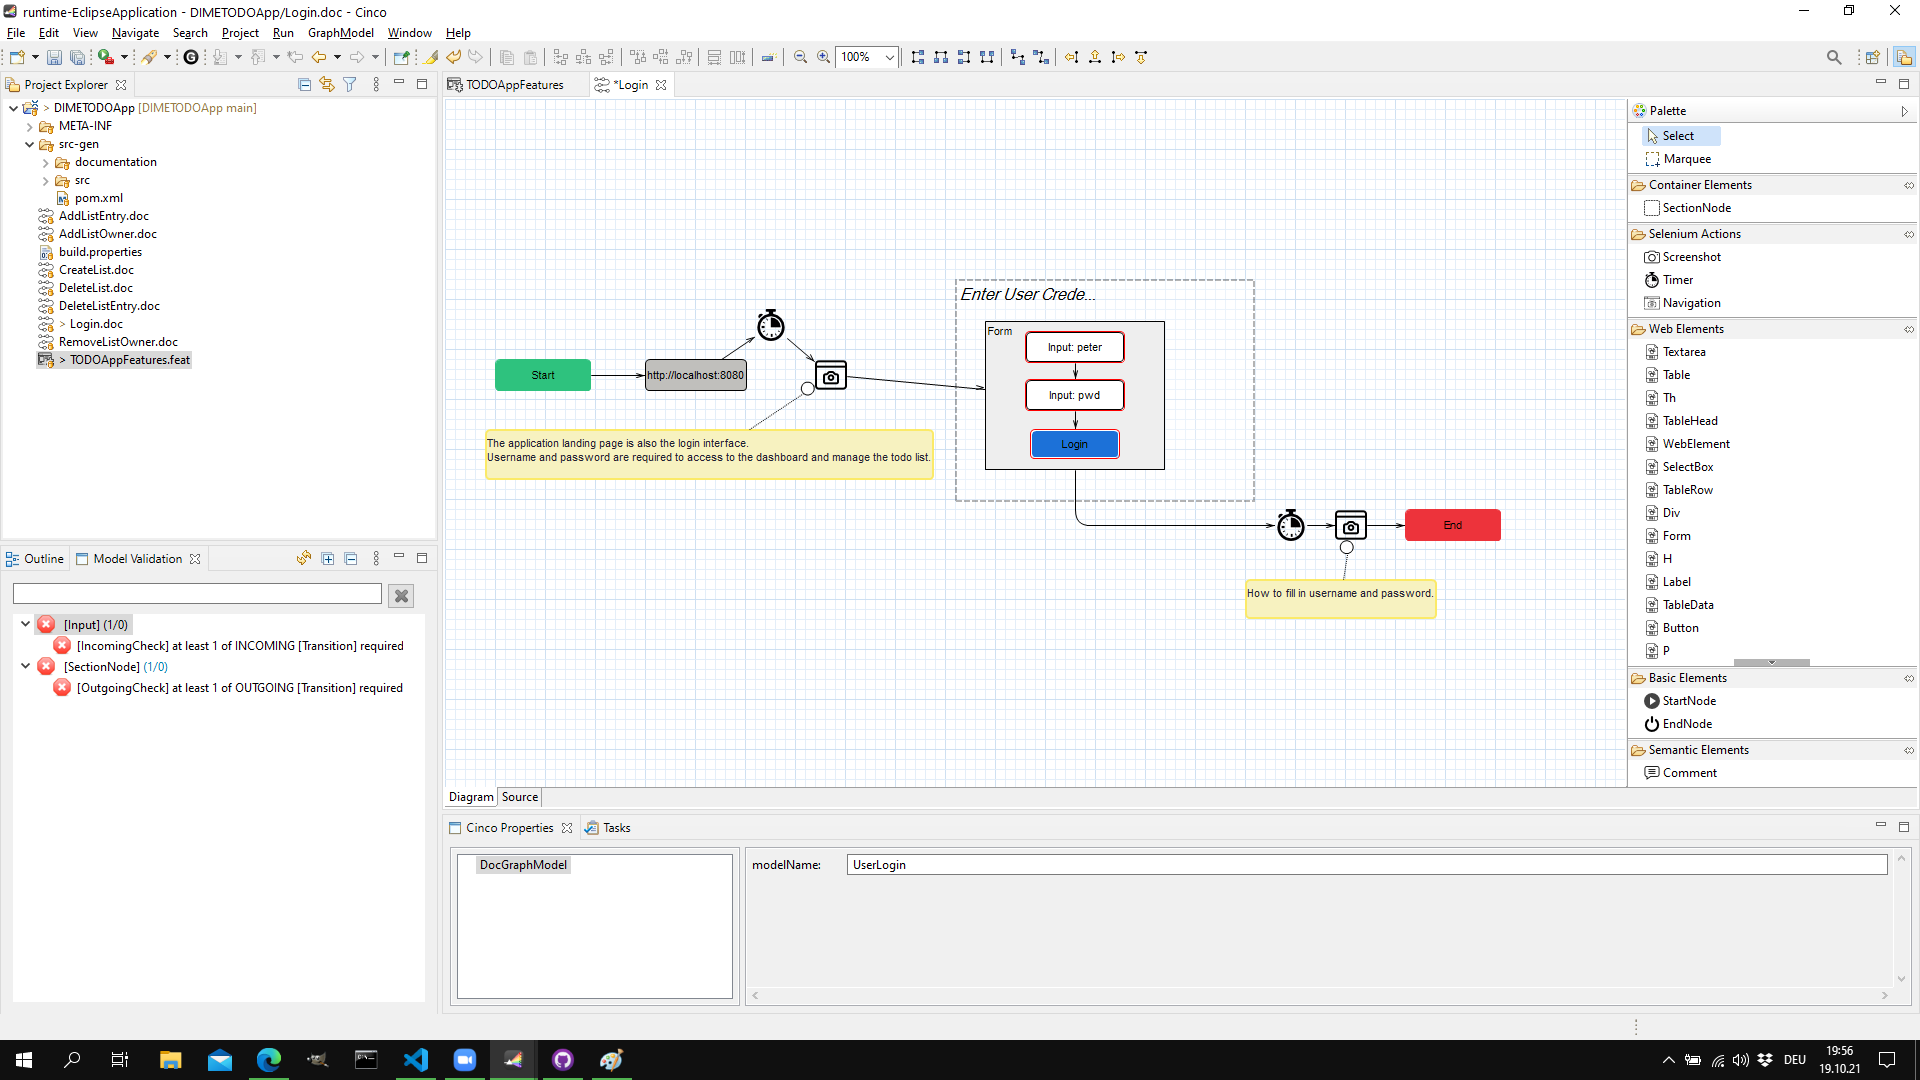
\includegraphics[width=\textwidth]{DocGraphModelChecks.png}
    \caption{\textsc{Cinco} Product Application - Graph model editor}\label{fig:graphDSL}
\end{figure}

All diagrams that are open in the editor are checked in the background for compliance with the requirements described on the metalevel using the \lstinline[language=MGL]{@mcam("check")} and shown in the Model Checking view right beneath the project explorer (4). There's also the \textsc{Cinco} property view (5) that displays the attributes and values of any selected element in the editor. This is where the developer can modify those values if the attribute field allows it.

The example model shown in Figure~\ref{fig:loginSeq} illustrate the sequence an end user would eventually undergo to login to the web application. Showing the web elements that will be interacted with and how combined into a logical sequence, they form a user workflow. The sequence begins with the start node then comes a navigation node with the link attribute pointing to \lstinline{http://localhost:8080}, the landing page of our TODO Web App in development.Next, the timer node waits explicitly for an amount of second the designer specified in the property view. The palette view presents a list of all the available graph model elements (see table~\ref{tab:listOfElements}). Since we specified two different \acrshortpl{mgl}, the list in the DocGraphModel differs from the one in the FeatureGraphModel. For instance, the DocGraphModel has a whole category for web elements specified, because the user action sequence is modeled using common UI elements of the web interface. On the other hand, the FeatureGraphModel is specially there to provide some start configuration (e.g. the path to the webdriver executable to be used), meaning that it regroups all the features modeled in every DocGraphModel, builds up both project structures mentioned before and triggers the code generation for every single one of them.

\begin{figure}[h]
    \centering
    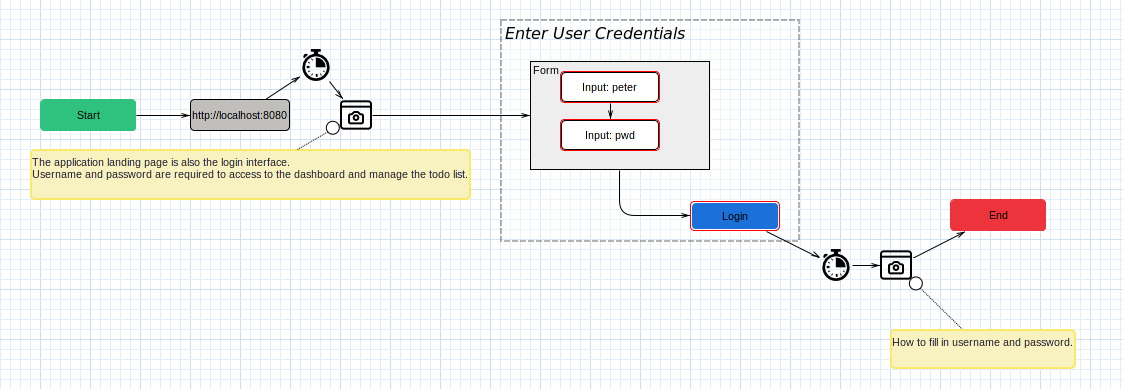
\includegraphics[width=\textwidth]{LoginSequence.png}
    \caption{Example of a user workflow: here the login sequence}
    \label{fig:loginSeq}
\end{figure}

\section{Feature Model Elements}\label{sec:FeatModElem}

The feature graph model is the application starting point. Here, the developer groups all the feature that needs to be documented in feature containers. Figure~\ref{fig:featGraph} depicts a portion of the features modeled for our TODO application. The important abilities of the web application are regrouped here: the ability to login, to create a new list, add a task to that list or remove it and lastly delete the whole list. Nonetheless, our TODO application offers the possibility to also add a new list owner, which already exist in the system as regular user. In order to have a reasonable size for the image, the last features are not shown on the picture. On the top left-hand corner you can see an property container holding the webdriver property, whose value is set to \lstinline[language=MGL]{FIREFOX}. This value will be assigned to the Selenium webdriver variable in the Java class. Remember that the executable file for the chosen webdriver muss already exist somewhere in file system and the path to it has to been specified here in the property view.

\begin{figure}[H]
    \centering
    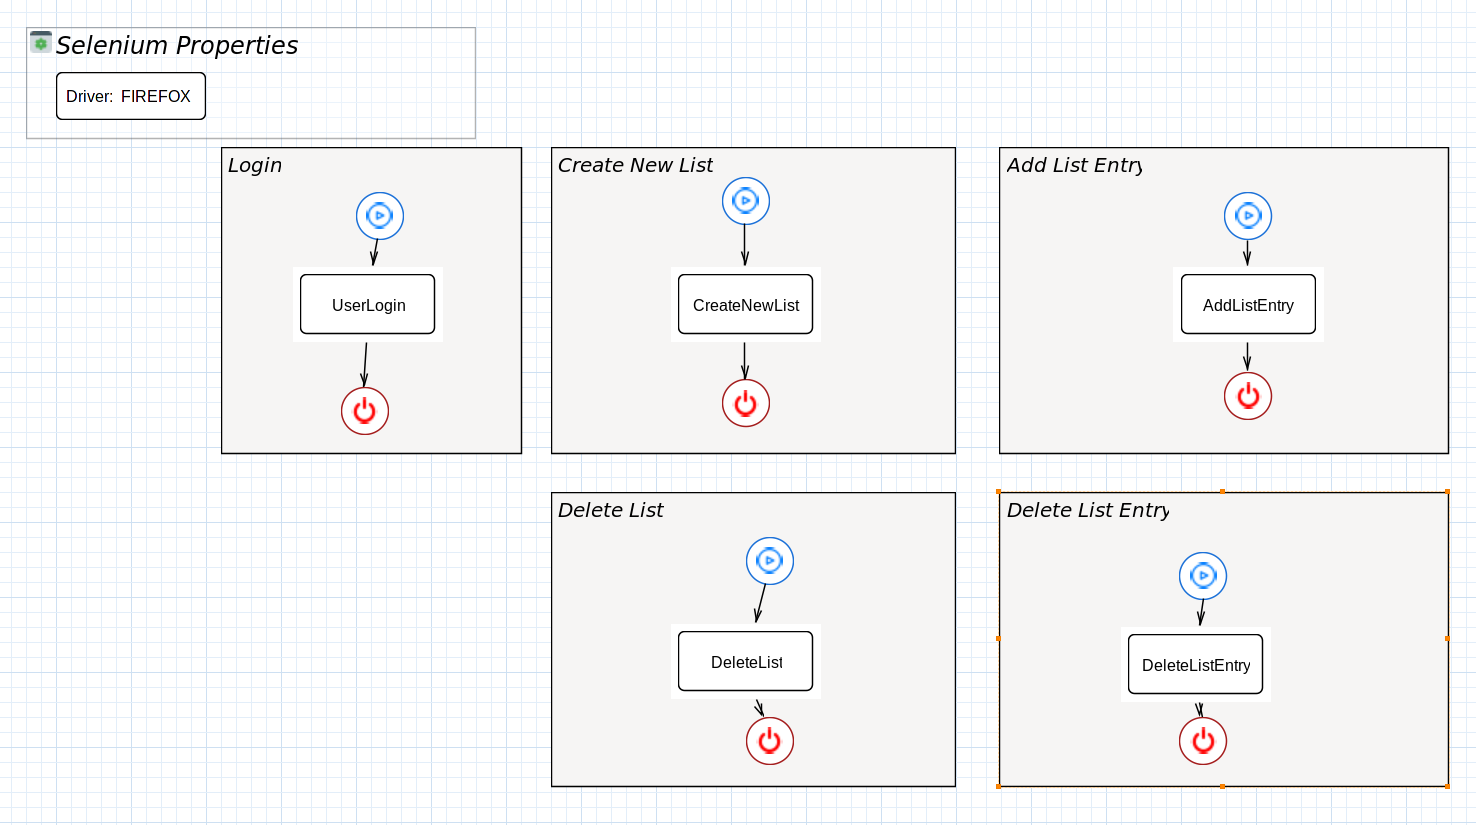
\includegraphics[width=\textwidth]{FeatureGraphModel2.png}
    \caption{\textsc{Cinco} product - Feature Graph Model with Feature Containers}
    \label{fig:featGraph}
\end{figure}

Even though the features are presented in logical workflow order, they still are independent from one another and will as well be generated independently. However, as mentioned in the previous chapter, this separation does not exclude reusability, since it is possible to integrate a whole DocGraphModel inside another one. considering, for instance, the CreateNewList feature, it requires the user to be logged in to be able to create a new tasks list. So the documentation developer does not have to repeat the login sequence inside the new, but can simply drag and drop the UserLogin.doc file inside the diagram of the new model graph and connect it within the sequence as if it were a regular graph node (see figure~\ref{fig:reusability}). Double-clicking on the imported subgraph leads directly to the original graph model. This double-click action has been implemented using the annotation \lstinline[language=MGL]{@doubleClickAction("info.scce.cinco.product.userdocumentation.action.DocNodeOpenSubmodel")}, where the DocNodeOpenSubmodel class holds the implementation logic.

The feature graph model contains also semantic elements, which are integrated in the existing featureContainer for simplicity's sake. Clicking on such a featureContainer opens up simultaneously the Cinco property view, where a multiline input field name description is found. This is where the documentation designer can enter some explanatory text to give meaning to the diagram elements and at the same time provide text content for the Markdown documentation files. Those information will be collected during the code generation process.

\section{User Action Model Elements}\label{sec:DocModElem}
In the user action model, just as the naming suggest, is where the action takes place. Here, the diagram editor has more elements to design the conceived user workflow: the graph elements categorized under ''Web Elements'', the Selenium actions and the comment node under the category ''Semantic Elements''.

One of the most import purposes of the web elements is to allow \acrshort{html} element to be addressed. This implies that appropriate actions can be applied to such representation of an \acrshort{html} element. considering for example the input field in the picture below, the action of inputting a text is made possible by provide a property variable \lstinline{content}, whose value is then display inside the node element (here i.e. ''Shopping''). The same holds true for button elements, which can be applied the click action or for selectboxes, which can be dropped down to reveal the options they contain, etc. In addition to that, all web element can be highlighted either by setting the \lstinline{highlighted} property to true or by letting the Highlight node amongst the Selenium actions take care of it.\unsure{unsure about this idea}

\begin{figure}[h]
    \centering
    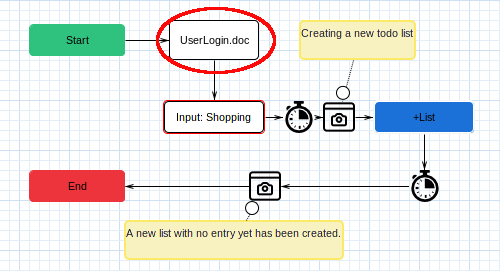
\includegraphics[width=\textwidth]{Reusability.png}
    \caption{\textsc{Cinco} product - Reusing Login graph model in the CreateNewList graph model}
    \label{fig:reusability}
\end{figure}

A particular element present in this diagram is the screenshot node, whose only task is to take a screen capture of the current state of the web application. Put in conjunction with the highlight functionality, screenshots with specific web elements highlighted (framed with a red border) can be created. That way, the documentation will contain visual help with the right emphasis on described \acrshort{html} element. Furthermore, the comment node allows the documentation creator to add descriptive text about the picture, that will be later added to the Markdown file as image caption. By specifying as different kind of edge for the comment node, we restricted its connection target to the screenshot node only. The idea behind is that all other diagram elements be commented on using the description property in the property view to avoid having diagrams filled with comment nodes.

One last particular element that need explanation is the timer node -- style by the chronometer. It belongs to the Selenium actions category and is intended to slow the webdriver down for a few seconds, while checking for a certain condition to become true before continuing. Said conditions are from the Selenium class named ExpectedConditions, from which we implemented a selected few applicable to our case, i.e. \lstinline{presenceOfElementLocated}, \lstinline{presenceOfAllElementsLocatedBy}, \lstinline{elementToBeClickable}, etc. If we take for instance the condition \lstinline{presenceOfElementLocated}, the timer holds the webdriver execution for 3 seconds, checking every 500 milliseconds if the target web element appears within the \acrshort{dom}

\section{Generation Process}\label{sec:GenProcess}

As mentioned before, the prominent feature of \textsc{Cinco} is the generate button. This allows the developer, after the modeled has been laid out without errors, to generate the a fully realized Selenium-Java application, which is going to execute the user sequence model just created. Figure~\ref{fig:genButton} shows where the generate button is located.

\begin{figure}[H]
    \centering
    
\includegraphics[width=\textwidth]{GenerateButtonHighlighted.png}
    \caption{\textsc{Cinco} product - generator button}
    \label{fig:genButton}
\end{figure}
